%; whizzy chapter
% -initex iniptex -latex platex -format platex -bibtex jbibtex -fmt fmt
% 以上 whizzytex を使用する場合の設定。


%     Tokyo Debian Meeting resources
%     Copyright (C) 2009 Junichi Uekawa
%     Copyright (C) 2012 Nobuhiro Iwamatsu

%     This program is free software; you can redistribute it and/or modify
%     it under the terms of the GNU General Public License as published by
%     the Free Software Foundation; either version 2 of the License, or
%     (at your option) any later version.

%     This program is distributed in the hope that it will be useful,
%     but WITHOUT ANY WARRANTY; without even the implied warranty of
%     MERCHANTABILITY or FITNESS FOR A PARTICULAR PURPOSE.  See the
%     GNU General Public License for more details.

%     You should have received a copy of the GNU General Public License
%     along with this program; if not, write to the Free Software
%     Foundation, Inc., 51 Franklin St, Fifth Floor, Boston, MA  02110-1301 USA

%  preview (shell-command (concat "evince " (replace-regexp-in-string "tex$" "pdf"(buffer-file-name)) "&"))
% 画像ファイルを処理するためにはebbを利用してboundingboxを作成。
%(shell-command "cd image200901; ebb *.png")

%%ここからヘッダ開始。

\documentclass[cjk,dvipdfmx,12pt]{beamer}
\usetheme{Tokyo}
\usepackage{monthlypresentation}
\usepackage{iwamatsu}

\setbeamertemplate{footline}{\hskip1mm\insertshortdate\hfill\hbox{\insertpagenumber /\insertdocumentendpage }\hspace*{1mm}\vskip1mm}

\newcommand<>{\fullsizegraphic}[1]{
  \begin{textblock*}{0cm}(-1cm,-3.78cm)
  \includegraphics[width=\paperwidth]{#1}
  \end{textblock*}
}

\newcommand<>{\minisectiontilte}[2]{
  {\fontsize{40pt}{40pt}\selectfont\color{#1}#2}
}

%  preview (shell-command (concat "evince " (replace-regexp-in-string "tex$" "pdf"(buffer-file-name)) "&")) 
%  presentation (shell-command (concat "xpdf -fullscreen " (replace-regexp-in-string "tex$" "pdf"(buffer-file-name)) "&"))
%  presentation (shell-command (concat "evince " (replace-regexp-in-string "tex$" "pdf"(buffer-file-name)) "&"))

%http://www.naney.org/diki/dk/hyperref.html
%日本語EUC系環境の時
\AtBeginDvi{\special{pdf:tounicode EUC-UCS2}}
%シフトJIS系環境の時
%\AtBeginDvi{\special{pdf:tounicode 90ms-RKSJ-UCS2}}

\title{第1回 Debian パッケージング道場 \\京都大学}
\subtitle{丸一日Debian漬けでDebianパッケージを作ってみる}
\author{岩松 信洋\\iwamatsu@debian.org}
\date{2013年2月9日}
\logo{
\includegraphics[width=8cm]{image200607/openlogo-light.eps}}

\begin{document}

\frame{\titlepage{}}

\begin{frame}{自己紹介とか、今日の予定などを書いてください}
ここに書いてください。
{
\url{http://debian-pkg-dojo.titanpad.com/1?}
}
\end{frame}

\begin{frame}{Debianパッケージ作成に詳しそうな人}

\begin{center}
\pause
\Huge{起立!}
\end{center}

\end{frame}

\begin{frame}{Debianパッケージ作成に詳しそうな人}
\begin{itemize}
\item この人たちににいろいろ聞いてください。
\end{itemize}
\end{frame}

\begin{frame}{自己紹介}

\begin{itemize}
\item 岩松 信洋 / Nobuhiro Iwamatsu
\item Twitter / @iwamatsu
\item Debian Project Official Developer
\item Linux kernel, Debian/SuperH, Bluetooth subsystem, Debian Science (OpenCV), Mozc, Erlang, etc...
\end{itemize}

\end{frame}

\begin{frame}{本日のスケジュール}
10:00 - 10:10 : 受付\\
10:10 - 10:20 : 諸注意 (佐々木さん)\\
10:20 - 11:00 : 基本的なパッケージの作成方法(前半)\\
11:00 - 11:10 : 休憩\\
11:10 - 12:00 : 基本的なパッケージの作成方法(後半)\\
      : 最新のパッケージング事情の説明と使い方\\
12:00 - 13:00 : 昼休み\\
13:00 -   : 作業開始\\
16:00 -   : 作業内容発表(一人二〜三分ぐらいで。)\\
16:30 - 17:00 : 後片付け\\
\end{frame}

\emtext{基本的なパッケージの作成方法}

\begin{frame}{目的}

\begin{itemize}
\item Debianパッケージ化されていないソフトウェアをパッケージ化して、
ビルドテストとパッケージの変更までを体験してみましょう。
\item DebianについてやDebianパッケージの素晴らしさについては語りませんのでご安心ください。
\end{itemize}
\end{frame}

\begin{frame}{資料}

ここにあります。
{
\url{http://tokyodebian.alioth.debian.org/pdf/debianmeetingresume201302-dojo.pdf}
}

\end{frame}

\begin{frame}{アジェンダ}
\begin{enumerate}
%\item Debian とは?
%\item Debian パッケージについて
\item 作業を始める前の準備をする
\item ソフトウェアの動作確認をする
\item パッケージの雛形を作成する
\item debian ディレクトリ以下ファイルを編集する
\item パッケージをビルドする
\item 作成されたファイルを確認する
\item パッケージをインストールする
\item パッケージのビルドテストをする
\item パッケージのインストール/アンインストールテストをする
\item ソフトウェアの変更し、パッケージ化する
\item 質疑応答
\end{enumerate}

\end{frame}

\begin{frame}{記号の説明}

\begin{itemize}
\item{\bf \$}\\コンソールからの入力を意味します。{\bf \$}は入力せずに
コマンドを入力してください。

\item {\bf \textbackslash}\\
コマンドラインやファイルの中身で{\bf \textbackslash}が書かれている場所は行が続いて
いる事を意味します。入力しないでください。 

\item {\bf ...}\\
省略を意味します。実際には長い出力がある場合に省略している場
合に利用しています。

\end{itemize}
\end{frame}

\begin{frame}{ルート権限について}

説明では、root権限を使った作業を行う場合があります。
その場合には sudo コマンドを使って作業をします。{\bf sudo}コマンドが必要な場
合にはコマンドラインの説明のところに{\bf sudo}を指定しています。

\end{frame}

\emtext{作業を始める前の準備をする}

\begin{frame}[containsverbatim]{ネットワーク設定}
\begin{itemize}
\item ネットワーク設定をしてください。

\begin{terminal}
$ ifconfg .....
\end{terminal}
%$
\end{itemize}

\end{frame}

\begin{frame}[containsverbatim]{パッケージメンテナ名の設定}
\begin{itemize}
\item パッケージメンテナの名前とメールアドレスを環境変数に設定します。
\item 適当なエディタを使って、{\bf $\sim$/.bashrc} に以下の例のように追記して
保存してください。

\begin{terminal}
export DEBFULLNAME="Nobuhiro Iwamatsu"
export DEBEMAIL=iwamatsu@debian.org
\end{terminal}
%$
\end{itemize}

\end{frame}

\begin{frame}[containsverbatim]{パッケージメンテナ名の設定}
保存できたら、ターミナルを起動し、
\begin{terminal}
$ source ~/.bashrc
\end{terminal}
%$
を実行してください。

\end{frame}

\begin{frame}[containsverbatim]{パッケージビルドに必要なパッケージのインストール}

パッケージのビルドに必要なパッケージのインストールをします。
{\bf packaging-dev}パッケージをインストールしてください。

\begin{terminal}
$ sudo apt-get install packaging-dev
\end{terminal}
%$

\end{frame}

\begin{frame}[containsverbatim]{パッケージビルドに必要なパッケージのインストール}

{\bf packaging-dev} はメタパッケージ
%\footnote{他のパッケージに依存するだけのパッケージ}
で、インストールすることによってDebianパッケージに必要なパッケージがインストールされます。

\begin{itemize}
\item build-essential
\item debhelper
\item devscripts
\item dput または dupload
\item lintian
\item pbuilder または cowbuilder または sbuild\\
\item quilt
\end{itemize}

\end{frame}

\begin{frame}[containsverbatim]{パッケージ化するソフトウェア}

\begin{itemize}
\item C++ で書いた適当なソフトウェアを用意しました。
\item コンパイルに必要なソフトウェアやライブラリ
がインストールされている場合には、{\bf ./configure ; make ; sudo make install} 
を実行することでコンパイルおよびインストールまでができるようになっています。
\item サンプルプログラム\\
  \url{http://people.debian.org/~iwamatsu/dpd/hello-cwidget-20120922.tar.gz}

\item このソフトウェアをDebianパッケージ化してみます。
\end{itemize}

\end{frame}

\begin{frame}[containsverbatim]{パッケージ化するソフトウェア}

ダウンロードして、適当なディレクトリに展開します。

\begin{terminal}
$ mkdir -p ~/debian/dojo/work
$ cd ~/debian/dojo/work
$ wget http://people.debian.org/~iwamatsu/dpd/\
    hello-cwidget-20120922.tar.gz
$ tar -xzf hello-cwidget-20120922.tar.gz
$ ls
hello-cwidget-20120922.tar.gz
hello-cwidget-20120922
\end{terminal}
%$
\end{frame}

\emtext{ソフトウェアの動作確認をする}

%\begin{frame}{ソースを読んでみる}
%どのようなソフトウェアなのか理解するためにもパッケージング化する前に
%ソースコードを読んで、ソフトウェアの中身を理解しておきましょう。
%
%\end{frame}


\begin{frame}[containsverbatim]{ソフトウェアをコンパイルしてみる}

\begin{itemize}
\item コンパイルできない/動作しないプログラムをパッケージ化してもしょうがないので、動作確認をします。
\item まず最低限コンパイルに必要なパッケージ {\bf build-essential} をインストールします。
\item インストールしていない場合には以下のように実行してインストールしてください。

\begin{terminal}
$ sudo apt-get install build-essential
\end{terminal}
%$

\end{itemize}
\end{frame}

\begin{frame}[containsverbatim]{ソフトウェアをコンパイルしてみる}

先ほど解凍したディレクトリに移動します。
移動した後、{\bf configure}を実行します。
\begin{terminal}
$ cd hello-cwidget-20120922
$ ./configure
\end{terminal}
%$

\end{frame}

\begin{frame}[containsverbatim]{ソフトウェアをコンパイルしてみる}

\begin{terminal}
$ ./configure
...
Alternatively, you may set the environment variables
SIGC_CFLAGS
and SIGC_LIBS to avoid the need to call pkg-config.
See the pkg-config man page for more details.
...
\end{terminal}
%$

\end{frame}

\begin{frame}[containsverbatim]{ソフトウェアをコンパイルしてみる}

\begin{terminal}
$ ./configure
...
Alternatively, you may set the environment variables
SIGC_CFLAGS
{\color{red}and SIGC_LIBS to avoid the need to call pkg-config.}
See the pkg-config man page for more details.
...
\end{terminal}
%$

実行するとエラーになります。
{\bf pkg-config}コマンドがなくてエラーになっている事がわかります。
{\bf pkg-config}コマンドはどのパッケージで提供されているのでしょうか。

\end{frame}

\begin{frame}[containsverbatim]{ソフトウェアをコンパイルしてみる}

\begin{itemize}
\item Debianで特定のコマンドやファイルが提供されているパッケージを探すには、{\bf apt-file}コマンドを利用します。
\item apt-file コマンドは{\bf apt-file}パッケージで提供されています。インストールしましょう。
\item インストールできたら、{\bf sudo apt-file update}を実行し、検索用のデータベースを構築します。
\end{itemize}

\begin{terminal}
$ sudo apt-get update
$ sudo apt-get install apt-file
$ sudo apt-file update
\end{terminal}
%$

\end{frame}

\begin{frame}[containsverbatim]{ソフトウェアをコンパイルしてみる}

今回は{\bf pkg-config}コマンドがないので以下のように実行し、提供されているパッケージを
検索します。

\begin{terminal}
$ apt-file search pkg-config
\end{terminal}
%$

\end{frame}

\begin{frame}[containsverbatim]{ソフトウェアをコンパイルしてみる}

\begin{terminal}
$ apt-file search pkg-config
{\color{red}pkg-config: /usr/bin/pkg-config}
pkg-config: /usr/share/doc/pkg-config/AUTHORS
pkg-config: /usr/share/doc/pkg-config/NEWS.gz
.....
ruby-pkg-config: /usr/share/doc/ruby-pkg-config/copyright
zsh: /usr/share/zsh/functions/Completion/Unix/_pkg-config
zsh-beta: /usr/share/zsh-beta/functions/Completion/Unix/_pkg-config
\end{terminal}
%$

実行すると、指定したファイルを提供しているパッケージ名が出力されます。
結果を確認すると、{\bf pkg-config}パッケージで提供されていることが分かります。

\end{frame}

\begin{frame}[containsverbatim]{ソフトウェアをコンパイルしてみる}

{\bf pkg-config} コマンドが提供されているパッケージが{\bf pkg-config}パッケージとわかったので、
インストールします。

\begin{terminal}
$ sudo apt-get install pkg-config
\end{terminal}
%$

\end{frame}

\begin{frame}[containsverbatim]{ソフトウェアをコンパイルしてみる}

再度{\bf configure}を実行してみましょう。
\begin{terminal}
$ ./configure
\end{terminal}
%$

\end{frame}

\begin{frame}[containsverbatim]{ソフトウェアをコンパイルしてみる}

\begin{terminal}
$ ./configure
...
{\color{red}No package 'sigc++-2.0' found}

Consider adjusting the PKG_CONFIG_PATH environment variable if you
installed software in a non-standard prefix.
...
\end{terminal}
%$

次は{\bf sigc++-2.0}が見つからないようです。

\end{frame}

\begin{frame}[containsverbatim]{ソフトウェアをコンパイルしてみる}

先ほどと同じように{\bf apt-file}を利用して検索し、インストールします。

\begin{terminal}
$ apt-file search sigc++-2.0.pc
libsigc++-2.0-dev: /usr/lib/x86_64-linux-gnu/pkgconfig/sigc++-2.0.pc
$ sudo apt-get install libsigc++-2.0-dev 
\end{terminal}
%$

\end{frame}

\begin{frame}[containsverbatim]{ソフトウェアをコンパイルしてみる}

再度 configure を実行します。
\begin{terminal}
$ ./configure
...
checking for CWIDGET... configure: error: Package 
requirements(cwidget) were not met:

{\color{red}No package 'cwidget' found}

Consider adjusting the PKG_CONFIG_PATH environment 
variable if you installed software in a non-standard prefix.
...
\end{terminal}
%$

またエラーになります。今度は{\bf cwidget}足りないようです。

\end{frame}

\begin{frame}[containsverbatim]{ソフトウェアをコンパイルしてみる}

再度検索してインストールします。

\begin{terminal}
$ apt-file search cwidget.pc
libcwidget-dev: /usr/lib/pkgconfig/cwidget.pc
$ sudo apt-get install libcwidget-dev
\end{terminal}

\end{frame}

\begin{frame}[containsverbatim]{ソフトウェアをコンパイルしてみる}

再度{\bf configure}を実行します。

\begin{terminal}
$ ./configure
\end{terminal}
%$

\end{frame}

\begin{frame}[containsverbatim]{ソフトウェアをコンパイルしてみる}

\begin{terminal}
$ ./configure
...
config.status: creating Makefile
config.status: creating config.h
config.status: config.h is unchanged
config.status: executing depfiles commands
\end{terminal}
%$

{\bf configure}が正常に終了しました。

\end{frame}

\begin{frame}[containsverbatim]{ソフトウェアをコンパイルしてみる}

終了すると、{\bf Makefile}が作成されています。
{\bf make}を実行し、コンパイルします。

\begin{terminal}
$ ls
AUTHORS      README          configure
COPYING      __Makefile.am   configure.in
ChangeLog    __configure.in  depcomp
INSTALL      aclocal.m4      hello-cwidget.cc
{\color{red}Makefile}     autom4te.cache  install-sh
Makefile.am  config.h        missing
Makefile.in  config.h.in     stamp-h1
NEWS         config.log
NOTE         config.status
$ make
\end{terminal}
%$

\end{frame}

\begin{frame}[containsverbatim]{ソフトウェアをコンパイルしてみる}

\begin{terminal}
$ make
make  all-am
make[1]: ディレクトリ `/home/iwamatsu/debian/dojo/work/hello-cwidget-20120922' に入ります
g++ -DHAVE_CONFIG_H -I.    -I/usr/include/sigc++-2.0 -I/usr/lib/x86_64-linux-gnu/sigc++-2.0/include   -I/usr/include/sigc++-2.0 -I/usr/lib/x86_64-linux-gnu/sigc++-2.0/include -I/usr/lib/cwidget   -g -O2 -MT hello_cwidget-hello-cwidget.o -MD -MP -MF .deps/hello_cwidget-hello-cwidget.Tpo -c -o hello_cwidget-hello-cwidget.o `test -f 'hello-cwidget.cc' || echo './'`hello-cwidget.cc
mv -f .deps/hello_cwidget-hello-cwidget.Tpo .deps/hello_cwidget-hello-cwidget.Po
g++ -I/usr/include/sigc++-2.0 -I/usr/lib/x86_64-linux-gnu/sigc++-2.0/include   -I/usr/include/sigc++-2.0 -I/usr/lib/x86_64-linux-gnu/sigc++-2.0/include -I/usr/lib/cwidget   -g -O2   -o hello-cwidget hello_cwidget-hello-cwidget.o -lsigc-2.0   -lcwidget -lncursesw -lsigc-2.0   
make[1]: ディレクトリ `/home/iwamatsu/debian/dojo/work/hello-cwidget-20120922' から出ます
\end{terminal}
%$

コンパイルも正常に終了したので、試しに実行します。
\begin{terminal}
$ ./hello-cwidget
\end{terminal}
%$

\end{frame}

\begin{frame}[containsverbatim]{ソフトウェアをコンパイルしてみる}

図のような画面が表示されたでしょうか。

\begin{center}
\includegraphics[width=0.8\hsize]{image201209/hello-debain-big.eps}
\end{center}

\end{frame}

\begin{frame}[containsverbatim]{ソフトウェアをコンパイルしてみる}

\begin{itemize}
\item ここまではサンプルプログラムの動作確認です。
\item どのようなソフトウェアなのか理解するためにも、
パッケージ化する前にソースコード等を読んでおくこ
とをお勧めします。
\end{itemize}

\end{frame}

\emtext{Debianパッケージの雛形を作成する}

\begin{frame}[containsverbatim]{Debianパッケージの雛形を作成する}

\begin{itemize}
\item Debianパッケージはソースが格納されているディレクトリの中に
{\bf debian}ディレクトリを作成します。
\item その中にパッケージビルドスクリプトを置き、実行することによってビルドされます。
\end{itemize}

\end{frame}

\begin{frame}[containsverbatim]{Debianパッケージの雛形を作成する}

\begin{itemize}
\item これらを構成するファイルやスクリプトはある程度決まっているため、
雛形が用意されています。
\item この雛形を作成するのが{\bf dh\_make}コマンドです。
これは{\bf dh-make}パッケージで提供されています。
\end{itemize}

\end{frame}

\begin{frame}[containsverbatim]{Debianパッケージの雛形を作成する}

\begin{itemize}
\item 作業の前に一度{\bf hello-cwidget-20120922}ディレクトリを削除します。
今まで行った {\bf ./configure} コマンド等で不要なファイルが作成されているからです。
\item そして再度展開し、作成されたディレクトリに移動します。
\end{itemize}

\begin{terminal}
$ cd ..
$ rm -rf hello-cwidget-20120922
$ tar -xzf hello-cwidget-20120922.tar.gz
$ cd hello-cwidget-20120922
\end{terminal}
%$

\end{frame}

\begin{frame}[containsverbatim]{Debianパッケージの雛形を作成する}

{\bf dh-make}パッケージをインストールします。

\begin{terminal}
$ sudo apt-get install dh-make
\end{terminal}
%$

\end{frame}

\begin{frame}[containsverbatim]{Debianパッケージの雛形を作成する}

Debianパッケージの雛形の作成します。以下のコマンドを実行します。
\begin{terminal}
$ dh_make --createorig -s
\end{terminal}
%$

\begin{itemize}
\item {\bf \texttt{--}createorig}
オリジナルソースコードのtar.gzイメージを構築します。 
\item {\bf -s}
今回はシングルバイナリパッケージ(一つのソースコードから一つの
バイナリパッケージがビルドされる)なので{\bf -s} を指定します。
\end{itemize}

\end{frame}

\begin{frame}[containsverbatim]{Debianパッケージの雛形を作成する}

実行すると以下のようなメッセージが表示されるので、Enterキーを押します。

\begin{terminal}
$ dh_make --createorig -s
Maintainer name  : Nobuhiro Iwamatsu
Email-Address    : iwamatsu@debian.org 
Date             : Wed, 12 Sep 2012 12:46:24 +0900
Package Name     : hello-cwidget
Version          : 20120922
License          : blank
Type of Package  : Single
Hit <enter> to confirm: 
\end{terminal}
%$

\end{frame}

\begin{frame}[containsverbatim]{debianディレクトリ}
コマンドを実行すると、{\bf debianディレクトリ}が作成され、この中に
パッケージ作成に必要な雛形が作成されます。
以下に作成されるファイル一覧を示します。

\begin{itemize}
\item README.Debian  (Debianパッケージの README)
\item README.source  (ソースの情報を記述する)
\item changelog      (Debianパッケージのチェンジログ)
\item compat         (debhelperのAPIバージョンを指定する)
\item control        (Debianパッケージ情報)
\item copyright      (著作権情報)
\item dirs           (作成するディレクトリ名を指定する)
\item docs           (インストールするドキュメントファイルを指定する)
\end{itemize}

\end{frame}

\begin{frame}[containsverbatim]{debianディレクトリ}
\begin{itemize}
\item emacsen-install.ex (emacs 用設定ファイル)
\item emacsen-remove.ex  (emacs 用設定ファイル)
\item emacsen-startup.ex (emacs 用設定ファイル)
\item hello-cwidget.cron.d.ex (cron用)
\item hello-cwidget.default.ex (debfonf用)
\item hello-cwidget.doc-base.EX (doc-base用)
\item init.d.ex      (init.dを使うパッケージ用設定ファイル)
\item manpage.1.ex   (manpage の雛形)
\item manpage.sgml.ex(manpage の雛形)
\item manpage.xml.ex (manpage の雛形)
\item menu.ex        (メニューの雛形)

\end{itemize}
\end{frame}

\begin{frame}[containsverbatim]{debianディレクトリ}
\begin{itemize}
\item postinst.ex    (postinstメンテナファイルの雛形)
\item postrm.ex      (postrmメンテナファイルの雛形)
\item preinst.ex     (preinstメンテナファイルの雛形)
\item prerm.ex       (prermメンテナファイルの雛形)
\item rules          (パッケージビルドスクリプト)
\item source         (Debian ソースパッケージ情報を格納するディレクトリ)
\item format     (Debian ソースフォーマットを指定する)
\item watch.ex       (アップストリームチェック用ファイル)

\end{itemize}

\end{frame}


\begin{frame}[containsverbatim]{不要なファイルの削除}
今回のパッケージ化に必要ではないファイルを{\bf debian}ディレクトリ以下から削除
します。hello-cwidget は emacs や cron を使わないプログラムなので、基本ファイルのみ
(changelog、compat、control、copyright、rules、source)のみでよいでしょう。
%\footnote{必須ファイルはchangelog、control、copyright、rules です。}

\begin{terminal}
$ rm -rf debian/*.ex debian/*.EX \textbackslash
  debian/README.Debian \textbackslash
  debian/README.source debian/dirs debian/docs
\end{terminal}
%$

\end{frame}

\emtext{debian ディレクトリ以下ファイルの編集}

\begin{frame}[containsverbatim]{debian/changelogファイルの編集する}

\begin{itemize}
\item Debian パッケージの変更は全て簡潔に Debian changelog ファイル(debian/changelog)
に記載する必要があります。
\item フォーマットに関してはDebian policy 4.4 Debian changelog: debian/changelog を参照。
\end{itemize}

\end{frame}

\begin{frame}[containsverbatim]{debian/changelogファイルの編集する}

{\bf debian/changelog}ファイルには既に{\bf ITP}(Intent To Package)
のテンプレート書かれているので削除します。以下のように変更します。

\begin{terminal}
hello-cwidget (20120922-1) unstable; urgency=low

  * Initial release.

 -- Nobuhiro Iwamatsu <iwamatsu@debian.org>  Wed, 12 Sep 2012 12:46:24 +0900

\end{terminal}
%$

\end{frame}


\begin{frame}[containsverbatim]{ライセンスとコピーライトをチェックする}

\begin{itemize}

\item ソフトウェアをDebianパッケージにしてDebian にインストールする際、重要な点として
ソフトウェアのライセンスがあります。
\item そのソフトウェアのライセンスがDFSG(Debian Free Software Guideline)に適合するか
チェックする必要があり、同梱されているファイルを確認する必要があります。
%\item ほとんどの場合、ソースにはLICENCEファイルやCOPYINGファイルが提供されていますが、
%一部のファイルは違うライセンスが適用されている場合もあるためです。もちろんファイル毎に
%\item ライセンスが書かれておらず、LICENCEファイル等で包容的にライセンスを決めている場合
%もあります。

\end{itemize}

\end{frame}

\begin{frame}[containsverbatim]{ライセンスとコピーライトをチェックする}

\begin{itemize}
\item Debianでは簡易的にチェックするためのツールとして {\bf licensecheck}があります。
\item 実行するとファイルのライセンスを出力します。
{\bf \texttt{--c}opyright}オプションをつけた場合、コピーライトホルダも出力します。
{\bf -r}オプションは再帰チェックです。
\end{itemize}

\begin{terminal}
$ licensecheck -r .
\end{terminal}
%$

\end{frame}

\begin{frame}[containsverbatim]{ライセンスとコピーライトをチェックする}

\begin{terminal}
$ licensecheck -r .
hello-cwidget.cc: BSD (2 clause) 
$ licensecheck -r --copyright .
hello-cwidget.cc: BSD (2 clause) 
  [Copyright: HOLDERS AND CONTRIBUTORS / 2012 Nobuhiro Iwamatsu <iwamatsu@debian.org>]
\end{terminal}
%$

簡易的ではありますが hello-cwidget で提供されている hello-cwidget.cc
のライセンスは 2 clause BSD Licenseで、
コピーライトは {\bf 2012 Nobuhiro Iwamatsu $<$iwamatsu@debian.org$>$}
が持っていることが分かりました。
ツールに頼らず、実際にチェックもしておきましょう。

\end{frame}


\begin{frame}[containsverbatim]{debian/copyrightファイルの編集する}

\begin{itemize}
\item Debianパッケージには、著作権と配布条件のライセンス文書が元のままの形式で 
/usr/share/doc/package/copyright に収録されていなければいけません
(Debian policy 4.5 Copyright: debian/copyright)。
\item パッケージの著作権やライセンス情報を提供するファイルが debian/copyright ファイルとなります。
これはDEP5(Debian Enhancement Proposals 5 )というフォーマットに基づいて書きます。
\item フォーマットはヘッダ段落とファイル段落に分かれており、その中に項記述するが決まっています。

\end{itemize}

\end{frame}

\begin{frame}[containsverbatim]{debian/copyrightファイルの編集する}

DEP5 に基づいて、前で確認したソフトウェアのライセンス用に debian/changelog を変更します。
以下のような内容になります。

\begin{terminal}
Format: http://www.debian.org/doc/packaging-manuals/copyright-format/1.0/
Upstream-Name: hello-cwidget
Source: http://people.debian.org/~iwamatsu/dpd/

Files: *
Copyright: 2012 Nobuhiro Iwamatsu <iwamatsu@debian.org>
License: BSD-2-Clause license

Files: debian/*
Copyright: 2012 Nobuhiro Iwamatsu <iwamatsu@debian.org>
License: BSD-2-Clause license

License: BSD-2-Clause license
 Redistribution and use in source and binary forms, with or without
 modification, are permitted provided that the following conditions are 
 met:
 .
 * Redistributions of source code must retain the above copyright notice,
   this list of conditions and the following disclaimer.
 * Redistributions in binary form must reproduce the above copyright notice,
   this list of conditions and the following disclaimer in the documentation
   and/or other materials provided with the distribution.
 .
 THIS SOFTWARE IS PROVIDED BY THE COPYRIGHT HOLDERS AND CONTRIBUTORS "AS IS" 
 AND ANY EXPRESS OR IMPLIED WARRANTIES, INCLUDING, BUT NOT LIMITED TO, 
 THE IMPLIED WARRANTIES OF MERCHANTABILITY AND FITNESS FOR A PARTICULAR
 PURPOSE ARE DISCLAIMED. IN NO EVENT SHALL THE COPYRIGHT HOLDER OR CONTRIBUTORS
 BE LIABLE FOR ANY DIRECT, INDIRECT, INCIDENTAL, SPECIAL, EXEMPLARY, OR
 CONSEQUENTIAL DAMAGES (INCLUDING, BUT NOT LIMITED TO, PROCUREMENT OF SUBSTITUTE
 GOODS OR SERVICES; LOSS OF USE, DATA, OR PROFITS; OR BUSINESS INTERRUPTION)
 HOWEVER CAUSED AND ON ANY THEORY OF LIABILITY, WHETHER IN CONTRACT, STRICT
 LIABILITY, OR TORT (INCLUDING NEGLIGENCE OR OTHERWISE) ARISING IN ANY WAY OUT 
 OF THE USE OF THIS SOFTWARE, EVEN IF ADVISED OF THE POSSIBILITY OF SUCH DAMAGE.
\end{terminal}

\end{frame}


\begin{frame}[containsverbatim]{debian/rulesファイルの編集する}

\begin{itemize}
\item {\bf debian/rules}にはパッケージのビルド手順を書きます。
\item これはパッケージ作成補助ツールである debhelper を使って書くことが多いです。
\item {\bf ./configure ; make ; sudo make install}だけでコンパイルとインストールが
できるソフトウェアは以下の内容だけでパッケージのビルドができます。
\end{itemize}

\begin{terminal}
#!/usr/bin/make -f
%:
    dh $@
\end{terminal}
%$

\end{frame}

\begin{frame}[containsverbatim]{debian/controlファイルの編集する}

debian/control ファイルにはパッケージ全体の情報とビルドされるパッケージの情報を書きます。
(Chapter 5 - Control files and their fields)
まずパッケージ全体の情報を書いてみます。

\begin{terminal}
Source: hello-cwidget
Section: devel
Priority: extra
Maintainer: Nobuhiro Iwamatsu <iwamatsu@debian.org>
Build-Depends: debhelper (>= 9.0.0)
Standards-Version: 3.9.4
Homepage: http://people.debian.org/~iwamatsu/dpd/
\end{terminal}

\end{frame}

\begin{frame}[containsverbatim]{debian/controlファイルの編集する}

\begin{itemize}
\item Source \\
パッケージの元になるソースの名前を書きます。
\end{itemize}

\begin{terminal}
{\color{red}Source: hello-cwidget}
Section: devel
Priority: extra
Maintainer: Nobuhiro Iwamatsu <iwamatsu@debian.org>
Build-Depends: debhelper (>= 9.0.0)
Standards-Version: 3.9.4
Homepage: http://people.debian.org/~iwamatsu/dpd/
\end{terminal}

\end{frame}

\begin{frame}[containsverbatim]{debian/controlファイルの編集する}

\begin{itemize}
\item Section\\
パッケージを分類したアプリケーション分野を指定します。
\end{itemize}

\begin{terminal}
Source: hello-cwidget
{\color{red}Section: devel}
Priority: extra
Maintainer: Nobuhiro Iwamatsu <iwamatsu@debian.org>
Build-Depends: debhelper (>= 9.0.0)
Standards-Version: 3.9.4
Homepage: http://people.debian.org/~iwamatsu/dpd/
\end{terminal}

\end{frame}

\begin{frame}[containsverbatim]{debian/controlファイルの編集する}

\begin{itemize}
\item Priority\\
パッケージの優先度を指定します。
\end{itemize}

\begin{terminal}
Source: hello-cwidget
Section: devel
{\color{red}Priority: extra}
Maintainer: Nobuhiro Iwamatsu <iwamatsu@debian.org>
Build-Depends: debhelper (>= 9.0.0)
Standards-Version: 3.9.4
Homepage: http://people.debian.org/~iwamatsu/dpd/
\end{terminal}

\end{frame}

\begin{frame}[containsverbatim]{debian/controlファイルの編集する}

\begin{itemize}
\item Maintainer\\
パッケージメンテナの名前とメールアドレスを書きます。
\end{itemize}

\begin{terminal}
Source: hello-cwidget
Section: devel
Priority: extra
{\color{red}Maintainer: Nobuhiro Iwamatsu <iwamatsu@debian.org>}
Build-Depends: debhelper (>= 9.0.0)
Standards-Version: 3.9.4
Homepage: http://people.debian.org/~iwamatsu/dpd/
\end{terminal}

\end{frame}

\begin{frame}[containsverbatim]{debian/controlファイルの編集する}

\begin{itemize}
\item Build-Depends
パッケージを生成するときに利用するパッケージを指定します。debhelper は一番利用されているパッケージ作成補助ツールです。
\end{itemize}

\begin{terminal}
Source: hello-cwidget
Section: devel
Priority: extra
Maintainer: Nobuhiro Iwamatsu <iwamatsu@debian.org>
{\color{red}Build-Depends: debhelper (>= 9.0.0)}
Standards-Version: 3.9.4
Homepage: http://people.debian.org/~iwamatsu/dpd/
\end{terminal}

\end{frame}

\begin{frame}[containsverbatim]{debian/controlファイルの編集する}

\begin{itemize}
\item Standards-Version\\
パッケージが準拠しているDebianポリシーマニュアルのバージョンを指定します。現在の最新バージョンは3.9.4です。
\end{itemize}

\begin{terminal}
Source: hello-cwidget
Section: devel
Priority: extra
Maintainer: Nobuhiro Iwamatsu <iwamatsu@debian.org>
Build-Depends: debhelper (>= 9.0.0)
{\color{red}Standards-Version: 3.9.4}
Homepage: http://people.debian.org/~iwamatsu/dpd/
\end{terminal}

\end{frame}

\begin{frame}[containsverbatim]{debian/controlファイルの編集する}

\begin{itemize}
\item Homepage\\
ソースが入手できるWebサイトを書きます。
\end{itemize}

\begin{terminal}
Source: hello-cwidget
Section: devel
Priority: extra
Maintainer: Nobuhiro Iwamatsu <iwamatsu@debian.org>
Build-Depends: debhelper (>= 9.0.0)
Standards-Version: 3.9.4
{\color{red}Homepage: http://people.debian.org/~iwamatsu/dpd/}
\end{terminal}

\end{frame}

\begin{frame}[containsverbatim]{debian/controlファイルの編集する}

\begin{itemize}
\item 次にビルドされるパッケージの情報を書きます。
\item hello-cwidget では hello-cwidget というプログラムを提供するので、
hello-cwidget という一つのパッケージを提供するようにします。

\end{itemize}

各項目について説明します。

\end{frame}


\begin{frame}[containsverbatim]{debian/controlファイルの編集する}




\begin{itemize}

\item Package \\
パッケージ名を書きます。

\end{itemize}

\begin{terminal}
{\color{red}Package: hello-cwidget}
Architecture: any
Depends: \$\{shlibs:Depends\}, \$\{misc:Depends\}
Description: Debian Packaging Hands-on sample program
 This is sample program of Debian Hands-on with OSC2009
 Tokyo/Spring and Debian Packaging Dojo.
 This is very easy program that uses cwidget.
\end{terminal}

\end{frame}


\begin{frame}[containsverbatim]{debian/controlファイルの編集する}

\begin{itemize}

\item Architecture \\
ビルド可能なマシンアーキテクチャを指定します。

\end{itemize}

\begin{terminal}
Package: hello-cwidget
{\color{red}Architecture: any}
Depends: \$\{shlibs:Depends\}, \$\{misc:Depends\}
Description: Debian Packaging Hands-on sample program
 This is sample program of Debian Hands-on with OSC2009
 Tokyo/Spring and Debian Packaging Dojo.
 This is very easy program that uses cwidget.
\end{terminal}

\end{frame}

\begin{frame}[containsverbatim]{debian/controlファイルの編集する}

\begin{itemize}

\item Depends \\
依存しているパッケージを指定します。
{\bf \$\{shlibs:Depends\}, \$\{misc:Depends\}}はビルド
されたファイルから自動的に依存ファイルを検出し、依存パッケージ名に置換されます。

\end{itemize}

\begin{terminal}
Package: hello-cwidget
Architecture: any
{\color{red}Depends: \$\{shlibs:Depends\}, \$\{misc:Depends\}}
Description: Debian Packaging Hands-on sample program
 This is sample program of Debian Hands-on with OSC2009
 Tokyo/Spring and Debian Packaging Dojo.
 This is very easy program that uses cwidget.
\end{terminal}

\end{frame}


\begin{frame}[containsverbatim]{debian/controlファイルの編集する}

\begin{itemize}

\item Description \\
パッケージの説明を書きます。1行目は短い説明を書き、2行目以降により詳細な説明を書きます。
2行目以降は先頭に1文字空白を入れる必要があります。

\end{itemize}

\begin{terminal}
Package: hello-cwidget
Architecture: any
Depends: ${shlibs:Depends}, ${misc:Depends}
 {\color{red}This is sample program of Debian Hands-on with OSC2009
 Tokyo/Spring and Debian Packaging Dojo.
 This is very easy program that uses cwidget.}
\end{terminal}

\end{frame}


\emtext{パッケージをビルドする}

\begin{frame}[containsverbatim]{パッケージをビルドする}

パッケージのビルドには{\bf debuild}コマンドを使います。
debuild コマンドは{\bf devscripts}パッケージで提供されています。

\begin{terminal}
$ debuild -us -uc
\end{terminal}
%$

\begin{itemize}
\item {\bf -us}はソースパッケージにPGP署名しないというオプションです。
\item {\bf -uc} は .changes ファイルにPGP署名しないというオプションです。
\end{itemize}

\end{frame}

\begin{frame}[containsverbatim]{パッケージをビルドする}

\if0
\begin{terminal}
$ debuild -us -uc
...
dpkg-buildpackage: full upload (original source is included)
{\color{red}Now running lintian...
W: hello-cwidget: hardening-no-relro usr/bin/hello
W: hello-cwidget: new-package-should-close-itp-bug
W: hello-cwidget: binary-without-manpage usr/bin/hello-cwidget}
Finished running lintian.
\end{terminal}
%$
\fi

\begin{terminal}
$ debuild -us -uc
...
dpkg-buildpackage: full upload (original source is included)
{\color{red}Now running lintian...
W: hello-cwidget source: newer-standards-version 3.9.4 (current is 3.9.3)
W: hello-cwidget: new-package-should-close-itp-bug
W: hello-cwidget: binary-without-manpage usr/bin/hello-cwidget}
Finished running lintian.
\end{terminal}
%$

パッケージのビルドが成功すると最後に lintian というパッケージチェックツールが実行されます。
%いくつか警告が出ていますので説明しておきます。

\end{frame}

\if0
\begin{frame}[containsverbatim]{パッケージをビルドする}


\begin{itemize}
\item hardening-no-relro \\
RELocation 領域(Global Offset Table (GOT)など)がリードオンリーになってない、という警告。
\end{itemize}

\begin{terminal}
$ debuild -us -uc
...
dpkg-buildpackage: full upload (original source is included)
Now running lintian...
{\color{red}W: hello-cwidget: hardening-no-relro usr/bin/hello}
W: hello-cwidget: new-package-should-close-itp-bug
W: hello-cwidget: binary-without-manpage usr/bin/hello-cwidget
Finished running lintian.
\end{terminal}
%$

\end{frame}

\begin{frame}[containsverbatim]{パッケージをビルドする}

\begin{itemize}
\item new-package-should-close-itp-bug \\
ITP のバグ番号が changelog ファイルに書かれていないという警告です。
%新しいパッケージを作成し、Debianにインストールする場合には ITP(Intent To Package)
%というバグを登録し、Debianパッケージのchangelog ファイルにこのバグ番号
%を書くことによってパッケージのアップロード時に対象のバグが閉じられます。
%他にも方法がありますが、この方法がよく使われます。
\end{itemize}


\begin{terminal}
$ debuild -us -uc
...
dpkg-buildpackage: full upload (original source is included)
Now running lintian...
W: hello-cwidget: hardening-no-relro usr/bin/hello
{\color{red}W: hello-cwidget: new-package-should-close-itp-bug}
W: hello-cwidget: binary-without-manpage usr/bin/hello-cwidget
Finished running lintian.
\end{terminal}
%$

\end{frame}

\begin{frame}[containsverbatim]{パッケージをビルドする}

\begin{itemize}
\item binary-without-manpage usr/bin/hello \\
usr/bin/hello の man ファイルがないという警告です(Debian-policy 12.1)。
\end{itemize}


\begin{terminal}
$ debuild -us -uc
...
dpkg-buildpackage: full upload (original source is included)
Now running lintian...
W: hello-cwidget: hardening-no-relro usr/bin/hello
W: hello-cwidget: new-package-should-close-itp-bug
{\color{red}W: hello-cwidget: binary-without-manpage usr/bin/hello-cwidget}
Finished running lintian.
\end{terminal}
%$

\end{frame}
\fi

\emtext{作成されたファイルを確認する}

\begin{frame}{作成されたファイルを確認する}

{\bf debuild} を実行した後には Debianパッケージだけでなく、いくつかファイルが作成されています。

\begin{terminal}
hello-cwidget-20120922

hello-cwidget\_20120922-1.debian.tar.gz
hello-cwidget\_20120922-1.dsc
hello-cwidget\_20120922-1\_amd64.build
hello-cwidget\_20120922-1\_amd64.changes
hello-cwidget\_20120922-1\_amd64.deb
hello-cwidget\_20120922.orig.tar.gz
\end{terminal}
%$

\end{frame}

\begin{frame}{作成されたファイルを確認する}

\begin{itemize}
\item *.debian.tar.gz\\
Debianパッケージ用に修正したファイルをまとめたもの。debian ディレクトリ以下のファイルです。
\item *.dsc\\
Debian のソースパッケージを構成するための情報が書かれたファイルです。
\item *.orig.tar.gz\\
開発元のソースコードです。
\item *.build\\
ビルドログです。
\item *.changes\\
パッケージ作成後の情報が書かれたファイルです。
\item *.deb\\
Debian パッケージです。
\end{itemize}

\end{frame}

\begin{frame}[containsverbatim]{パッケージをインストールする}

パッケージが無事ビルドできたら、実際にインストールしてみます。
インストールには {\bf debi} コマンドを使ってインストールします。インストールし
たら、動作確認をしてみましょう。

\begin{terminal}
$ sudo debi 
$ which hello-cwidget
/usr/bin/hello-cwidget
$ hello-cwidget
\end{terminal}
%$

\end{frame}

\emtext{パッケージのビルドテストをする}
\section{パッケージのビルドテストをする}

\begin{frame}[containsverbatim]{パッケージのビルドテストをする}

\begin{itemize}
\item パッケージができた後はパッケージのテストを行います。
\item パッケージのビルドテストには{\bf pbuilder}を使います。
\item pbuilder は chroot を使って Debian OSとして必要な最低限の環境から
パッケージビルドを行うツールです。これによって、パッケージビルドに
必要なパッケージが漏れていないかチェックできます。
\end{itemize}
%また cowbuilder はchroot 環境を構築する時にcopy-on-writeを利用できるようにするツールを提供します。

\end{frame}

\begin{frame}[containsverbatim]{pbuilderパッケージのインストール}

{\bf pbuilder と cowbuilder}をインストールしていない人は以下のように
実行し、インストールします。

\begin{terminal}
$ sudo apt-get install pbuilder cowbuilder
\end{terminal}
%$

インストールが完了したら、pbuilder でcowbuilder を利用できるように、
pbuilder の設定ファイル({\bf $\sim$/.pbuilderrc})に以下の内容を追記します。

\begin{terminal}
PDEBUILD_PBUILDER=cowbuilder
\end{terminal}
%$
\end{frame}


\begin{frame}[containsverbatim]{pbuilder環境の構築}

ビルドテストを行う前にbaseシステムイメージを構築する必要があります。
以下のように実行します。

\begin{terminal}
$ sudo cowbuilder --create
\end{terminal}
%$

\end{frame}

\begin{frame}[containsverbatim]{パッケージのビルドテスト}

パッケージのビルドテストを行うには、対象とするDebianパッケージの
ソースが展開されたディレクトリで{\bf pdebuild}を実行します。

\begin{terminal}
$ pdebuild
...
\end{terminal}
%$

\end{frame}


\begin{frame}[containsverbatim]{pdebuild によるパッケージビルドエラー}

実行するとビルドエラーになります。
なぜエラーになるのでしょうか。考えてみましょう。

\end{frame}


\begin{frame}[containsverbatim]{再ビルドテスト}
エラーになる理由は先にインストールしたパッケージ{\bf libcwidget-dev}をパッケー
ジビルド時の依存関係を記述するフィールド{\bf Build-Depends}に追加してい
ないためです。追加して見ましょう。

\begin{terminal}
Source: hello-cwidget
Section: devel
Priority: extra
Maintainer: Nobuhiro Iwamatsu <iwamatsu@debian.org>
Build-Depends: debhelper (>= 9.0.0), {\color{red}libcwidget-dev}
Standards-Version: 3.9.4
Homepage: http://people.debian.org/~iwamatsu/dpd/
\end{terminal}

\end{frame}


\begin{frame}[containsverbatim]{再ビルドテスト}
追加したら{\bf pdebuild}を実行し、再ビルドします。
今度はビルドができるはずです。

\begin{terminal}
$ pdebuild
...
\end{terminal}
%$

\end{frame}

\emtext{パッケージのインストール/アンインストールテスト}

\begin{frame}[containsverbatim]{パッケージのインストール/アンインストールテストをする}

パッケージがビルドできただけでは喜んではいけません。インストール/アンイ
ンストールのテストも行いましょう。
パッケージのインストール/アンインストールのテストには{\bf piuparts}パッ
ケージを使います。
\end{frame}


\begin{frame}[containsverbatim]{piupartsのインストール}
以下のように実行し、インストールします。

\begin{terminal}
$ sudo apt-get install piuparts
\end{terminal}
%$

\end{frame}

\begin{frame}[containsverbatim]{パッケージのインストール/アンインストールテスト}
piupartsもpbuilderと同様に最低限の環境からのインストールをチェックします。

\begin{terminal}
$ sudo piuparts -d unstable \textbackslash
  ../hello-cwidget_20120922-1_amd64.deb
...
0m41.9s DEBUG: Removed directory tree at /tmp/tmpHliOKO
0m41.9s INFO: PASS: All tests.
0m41.9s INFO: piuparts run ends.
\end{terminal}
%$

その他詳しい使い方は マニュアルを参照してください。
\end{frame}

\emtext{ソフトウェアの変更をする}

\begin{frame}{ソフトウェアの変更をする}

hello-cwidgetを実行して、違和感のある方がおられたと思います。
そう、{\bf Debian}が{\bf Debain}になっていました。これはよくないので修正しましょう。

\begin{center}
\includegraphics[width=0.8\hsize]{image201209/hello-debain-big.eps}
\end{center}

\end{frame}

\begin{frame}{ソフトウェアの変更をする}

Debian source-format バージョン 3.0からは{\bf quilt}によるパッチシステム
を使うことが推奨されています。
また、これを使うためのツールが整備されています。
この方法について説明します。

\end{frame}


\begin{frame}[containsverbatim]{ソフトウェアの変更をする}
早速ファイルを修正します。変更したい箇所は Typo なので grep 等で検索すると
よいでしょう。

\begin{terminal}
$ grep -r Debain *
hello-cwidget.cc:dialogs::ok(L"Hello, Debain Dojo!",
\end{terminal}
%$

\end{frame}

\begin{frame}[containsverbatim]{修正した箇所をパッチにする}

\begin{enumerate}
\item 修正した箇所をパッチするには {\bf dpkg-source} コマンドに {\bf \texttt{--}commit}
オプションをつけて実行します。
\item 実行すると保存するファイル名を聞かれるので、適当な名前をつけてエンターキーを押します。
\item パッチにファイル変更内容等が書かれたファイルが表示されますので、
この内容を適当に変更して保存します。\\
\item 保存すると debian/patches ディレクトリにパッチが保存され、debian/patches/series
ファイルに適用するパッチとして登録されます。
\end{enumerate}

\begin{terminal}
$ dpkg-source --commit
dpkg-source: info: local changes detected, the \textbackslash
modified files are:
 hello-cwidget-20120922/hello-cwidget.cc
Enter the desired patch name: fix-typo
\end{terminal}
%$

\end{frame}

\begin{frame}[containsverbatim]{修正した箇所をパッチにする}

作成されるパッチの内容は以下のようになります。

\begin{terminal}
Description: <short summary of the patch>
 TODO: Put a short summary on the line above and replace this paragraph
 with a longer explanation of this change. Complete the meta-information
 with other relevant fields (see below for details). To make it easier, the 
 information below has been extracted from the changelog. Adjust it or drop
 it. 
 .
 hello-cwidget (20120922-1) unstable; urgency=low
 .
   * Initial release.
Author: Nobuhiro Iwamatsu <iwamatsu@debian.org>

---
The information above should follow the Patch Tagging Guidelines, please
checkout http://dep.debian.net/deps/dep3/ to learn about the format. Here
are templates for supplementary fields that you might want to add:

Origin: <vendor|upstream|other>, <url of original patch>
Bug: <url in upstream bugtracker>
Bug-Debian: http://bugs.debian.org/<bugnumber>
Bug-Ubuntu: https://launchpad.net/bugs/<bugnumber>
Forwarded: <no|not-needed|url proving that it has been forwarded>
Reviewed-By: <name and email of someone who approved the patch>
Last-Update: <YYYY-MM-DD>

--- hello-cwidget-20120922.orig/hello-cwidget.cc
+++ hello-cwidget-20120922/hello-cwidget.cc
@@ -8,7 +8,7 @@ int main(int argc, char **argv)
    toplevel::init();
 
    widgets::widget_ref dialog =
-       dialogs::ok(L"Hello, Debain Dojo!",
+       dialogs::ok(L"Hello, Debian Dojo!",
            util::arg(sigc::ptr_fun(toplevel::exitmain)));
 
    toplevel::settoplevel(dialog);
...

dpkg-source: info: local changes have been recorded in a new patch: hello-cwidget-20120922/debian/patches/fix-typo
\end{terminal}
%$

\end{frame}

\begin{frame}[containsverbatim]{修正した箇所をパッチにする}

\begin{itemize}
\item Description\\
パッチの説明を書きます。
\item Origin\\
パッチの提供者を書きます。また開発元や他の」サイトからパッチ
を持ってきているとき、そのURLを書きます。
\item Bug\\
開発元のBTS登録されているバグ番号がある場合に書きます。
\item Bug-Debian\\
Debianのバグ番号のURLを書きます。
\end{itemize}

\end{frame}

\begin{frame}[containsverbatim]{修正した箇所をパッチにする}

\begin{itemize}
\item Bug-Ubuntu\\
Ubuntuのバグ番号のURLを書きます。
\item Forwarded\\
バグの転送先、その必要の可否を書きます。
\item Reviewed-By\\
パッチのレビュアを書きます。
\item Last-Update\\
パッチの更新日を書きます。
\item Applied-Upstream \\
開発元で適用された/されている場合、そのソースを示すURLを書きます。
\end{itemize}

\end{frame}

\begin{frame}[containsverbatim]{修正した箇所をパッチにする}

パッチの内容を修正すると以下のようになります。

\begin{terminal}
Description: Fixed message in dialog
 This patch is fixed typo form Debain to Debian.
Forwarded: not-needed
Origin: other
Author: Nobuhiro Iwamatsu <iwamatsu@debian.org>
Last-Update: 2012/09/22

--- hello-cwidget-20120922.orig/hello-cwidget.cc
+++ hello-cwidget-20120922/hello-cwidget.cc
@@ -8,7 +8,7 @@ int main(int argc, char **argv)
    toplevel::init();
 
    widgets::widget_ref dialog =
-       dialogs::ok(L"Hello, Debain Dojo!",
+       dialogs::ok(L"Hello, Debian Dojo!",
            util::arg(sigc::ptr_fun(toplevel::exitmain)));
 
    toplevel::settoplevel(dialog);
\end{terminal}
%$

\end{frame}

\begin{frame}[containsverbatim]{修正した箇所をパッチにする}

debian/patches/series ファイルを確認してみます。

\begin{terminal}
$ cat debian/patches/series 
fix-typo
\end{terminal}
%$

\end{frame}

\begin{frame}[containsverbatim]{差分を適用したパッケージをビルドする}

差分を適用したパッケージをビルドするには通常のパッケージビルドと変わりません。
{\bf debuild}コマンドを使ってビルドします。

debian/patches/series に書かれているパッチが順に適用され、
パッケージがビルドされます。

\begin{terminal}
$ debuild -us -uc
....
\end{terminal}
%$

\end{frame}

\begin{frame}[containsverbatim]{差分を適用したパッケージをビルドする}

作成されたパッケージをインストールして動作確認してみましょう。
Typoは治っているでしょうか。

\begin{terminal}
$ sudo debi
....
$ hello-cwidget
\end{terminal}
%$

\end{frame}

\begin{frame}[containsverbatim]{差分を適用したパッケージをビルドする}

\begin{center}
\includegraphics[width=0.8\hsize]{image201209/hello-debian-big.eps}
\end{center}

この後には{\bf pbuilder}と{\bf piuparts}を使ってパッケージのテストを行う事も忘れずに。

\end{frame}


\begin{frame}[containsverbatim]{質疑応答}
以上で、「基本的なパッケージの作成方法」は終了です。何か質問等はありますか?
\end{frame}

\if0
\begin{frame}{今回取り上げなかった事}
\end{frame}

\begin{frame}[containsverbatim]{どのパッケージをBuild-Depends に指定すればいいのか}

{\bf dpkg-depcheck}を使うと処理で必要だったライブラリやツールが提供されている
パッケージを出力してくれます。

\begin{terminal}
$ dpkg-depcheck -a make
make  all-am
...
Packages used:
  g++-4.7
  libtinfo5:amd64
  libselinux1:amd64
  zlib1g:amd64
  libsigc++-2.0-dev:amd64
  bash
...
\end{terminal}
%$

\end{frame}


\begin{frame}[containsverbatim]{インストール/アンインストール時に何かを行う}

パッケージインストールするとき、展開するだけでは不十分な時があります。
サービスを開始停止させたい場合がよい例です。
これらは メンテナスクリプト (preinst, postinst, prerm, postrm) で行います。
以下のドキュメントを参照してください。
\begin{itemize}
\item Debian Policy, 第6章
\item Debian Developer’s Reference,  6章
\item debconf-devel(7) (debconf-doc で提供されています)
\end{itemize}

\end{frame}
\fi

\emtext{最新のパッケージング事情の説明と使い方}


\emtext{debhelper 7 / 9}

\begin{frame}[containsverbatim]{debhelper 7 / 9}
よく利用されるパッケージ作成補助ツールにdebhelplerがあります。 バージョン7 から
大幅な改良が行われました。これらについて簡単に紹介します。

\end{frame}

\begin{frame}[containsverbatim]{各処理の隠蔽化}
バージョン7から Debianパッケージの作成に必要な処理が隠蔽化され、シンプルに debian/rules ファイルが
書けるようになりました。

\end{frame}

\begin{frame}[containsverbatim]{debian/rules の必須ターゲット}

\begin{center}
\includegraphics[width=1.0\hsize]{image201302/rules.eps}
\end{center}

\end{frame}

\begin{frame}[containsverbatim]{debian/rules の必須ターゲット}

\begin{itemize}
\item clean ターゲット\\
ビルドツリー内にある、生成されたりコンパイルされたりしたファイルを削除します。

\item build ターゲット\\
ビルドツリー内にプログラムやドキュメントをビルドします。

\begin{itemize}
\item build-arch ターゲット\\
ビルドツリー内にアーキテクチャーに依存したコンパイルしたプログラムをビルドします。

\item build-indep ターゲット\\
ビルドツリー内にアーキテクチャーに依存しないファイル(ドキュメントなど)をビルドします。
\end{itemize}

\end{itemize}

\end{frame}

\begin{frame}[containsverbatim]{debian/rules の必須ターゲット}

\begin{itemize}
\item install ターゲット: \\
debianディレクトリー以下にある各バイナリーパッケージのファイルツリーにファイルをインストールします。

\item binary ターゲット: 全てのバイナリーパッケージを作ります。
\begin{itemize}
\item binary-arch ターゲット\\
アーキテクチャーに依存したバイナリーパッケージ (Architecture: any)を作ります。

\item binary-indep ターゲット
アーキテクチャーに依存しないパッケージ (Architecture: all) を作ります。
\end{itemize}
\end{itemize}
\end{frame}

\begin{frame}[containsverbatim]{各処理の隠蔽化}

以前: 
\begin{terminal}
...
build: build-stamp
build-stamp:
    dh_testdir
    # Add here commands to compile the package.
    $(MAKE) 

    touch build-stamp
....
\end{terminal}
%$

バージョン7以降:
\begin{terminal}
%:                              
    dh $@
\end{terminal}
%$

\end{frame}

\begin{frame}[containsverbatim]{各処理の隠蔽化}

パッケージをビルドすると分かりますが、バージョン7以降では各ターゲットで
必要な処理に対応する debhelper スクリプトが呼ばれるようになっています。

\begin{terminal}
$ debuild -us -uc
...
 dh_auto_test
   fakeroot debian/rules binary
 dh binary
    dh_testroot
    dh_prep
    dh_installdirs
    dh_auto_install
...
\end{terminal}
%$

\end{frame}

\begin{frame}[containsverbatim]{各処理の隠蔽化}

\begin{itemize}
\item 各ターゲット内や各 debhelper スクリプトが呼ばれる前に処理を行いたい場合には、オーバライド機能
を使って各処理をオーバライドします。
\end{itemize}

{\bf dh\_auto\_test}を行う前に {\bf Foo}と出力したい場合:

\begin{terminal}
%:
    dh $@

{\color{red}override_dh_auto_test:}
    echo "Foo"
    dh_auto_test
\end{terminal}
%$

\end{frame}

\begin{frame}[containsverbatim]{サードパーティツール指定方法}

\begin{itemize}
\item 自分で dh\_* を作って、サードパーティツールとして利用できます。
\item debhelper 7 から {\bf \texttt{--}with}を使ってツールを指定する必要があります。
\end{itemize}

ruby のパッケージ補助ツールである dh\_ruby を使う例:
\begin{terminal}
%#! /usr/bin/make -f
%:
    dh $@ --buildsystem=ruby --with ruby 
\end{terminal}
%$

\end{frame}

\emtext{source 3.0}

\begin{frame}[containsverbatim]{source 3.0}

\begin{itemize}
\item Debian ソースパッケージのフォーマット”3.0 (uilt)"\\
squeeze から採用されています。
\item  以下の問題を解決するフォーマットです。

\begin{enumerate}
 \item アーカイブの圧縮形式に gzip しか使えない
 \item 複数のアーカイブで構成される上流のソースがそのまま扱えない
 \item メンテナが当てたソースへのパッチが全部つながってしまっている
 \item \verb|debian/| 以下にバイナリファイルが直接置けない
\end{enumerate}

\end{itemize}

\end{frame}

\begin{frame}[containsverbatim]{source 3.0}

"1.0" では、ソースパッケージは以下の3ファイルで構成されます。
\begin{itemize}
 \item \textit{packagename}\verb|-|\textit{upstreamversion}\verb|.orig.tar.gz|
 \item \textit{packagename}\verb|-|\textit{debianversion}\verb|.diff.gz|
 \item \textit{packagename}\verb|-|\textit{debianversion}\verb|.dsc|
\end{itemize}

正確には\verb|1.0|は2種類あり、上の通常のパッケージのほかに"Debian   
nativeな"パッケージがあります。Debian native パッケージは次の2ファイルで構成されます。
\begin{itemize}
 \item \textit{packagename}\verb|-|\textit{version}\verb|.tar.gz|
 \item \textit{packagename}\verb|-|\textit{version}\verb|.dsc|
\end{itemize}

\end{frame}

\begin{frame}[containsverbatim]{source 1.0}

\begin{itemize}
 \item \textit{packagename}\verb|-|\textit{upstreamversion}\verb|.orig.tar.gz|\\
上流の元のソースツリーが含まれます。

 \item \textit{packagename}\verb|-|\textit{debianversion}\verb|.diff.gz|\\
ソースパッケージからパッケージなどをビルドするのに必要なスクリ
プトなどが入った \verb|debian/| ディレクトリや、上流のソースに対するパッケージ
メンテナの変更が含まれます。
 \item \textit{packagename}\verb|-|\textit{debianversion}\verb|.dsc|\\
ソースパッケージのメタデータです。
\end{itemize}

\end{frame}

\begin{frame}[containsverbatim]{source 3.0}

\verb|3.0 (quilt)|は次の3つ以上のファイルで構成されます。
\begin{itemize}
 \item \textit{packagename}\verb|-|\textit{upstreamversion}\verb|.orig.tar.|\textit{ext}
 \item \textit{packagename}\verb|-|\textit{upstreamversion}\verb|.orig-|\textit{component}\verb|.tar.|\textit{ext}(任意)
 \item \textit{packagename}\verb|-|\textit{debianversion}\verb|.debian.tar.|\textit{ext}
 \item \textit{packagename}\verb|-|\textit{debianversion}\verb|.dsc|
\end{itemize}

なお、\verb|1.0|にあったDebian nativeパッケージに相当する\verb|3.0 (native)|は
次の2つのファイルで構成されます。
\begin{itemize}
 \item \textit{packagename}\verb|-|\textit{version}\verb|.tar.|\textit{ext}
 \item \textit{packagename}\verb|-|\textit{version}\verb|.dsc|
\end{itemize}

\end{frame}

\begin{frame}[containsverbatim]{source 3.0}

今後は "3.0 (quilt)"、"3.0 (native)"を使うようにしましょう。

\end{frame}

\emtext{hardening}

\begin{frame}[containsverbatim]{hardening}
次期リリース Debian 7.0から {\bf Security hardening build flags} を
有効にしたパッケージが提供されるようになります。

これはパッケージ構築時にセキュリティを強化するコンパイルフラグを(デフォルトで)有効にするというものです。現在、以下の4点を有効にする必要があります。

\begin{itemize}
  \item Format string checks( -Wformat -Werror=format-security )\\
  \item FORTIFY\_SOURCE \\
  \item -fstack-protector --param=ssp-buffer-size=4 \\
  \item -z,now,-z,relro \\
\end{itemize}

\end{frame}

\begin{frame}[containsverbatim]{hardening}

\begin{itemize}
\item これらのコンパイルオプションを自動的にCFLAGS変数等に設定する機構は今の所なく、
debian/rules に記述する必要があります。
\item いくつか方法がありますが、よく使われるのは{\bf dpkg-buildflags}でDebianで
推奨されるコンパイルオプションを取得し、各変数に設定するというものです。
\end{itemize}

\begin{terminal}
#!/usr/bin/make -f

CPPFLAGS:=$(shell dpkg-buildflags --get CPPFLAGS)
CFLAGS:=$(shell dpkg-buildflags --get CFLAGS)
CXXFLAGS:=$(shell dpkg-buildflags --get CXXFLAGS)
LDFLAGS:=$(shell dpkg-buildflags --get LDFLAGS)

%:
    dh $@
\end{terminal}
%$

\end{frame}

\begin{frame}[containsverbatim]{hardening}

その他の方法は\url{http://wiki.debian.org/Hardening}を参照してください。

\end{frame}

\begin{frame}[containsverbatim]{hardening}

hardening が有効なバイナリになっているか簡易的にチェックするためのツールがあります。
\begin{itemize}
\item hardening-check\\
バイナリからチェックする

\item blhc\\
ビルドログからチェックする

\end{itemize}

blhc によるチェック結果は buildlogcheck\footnote{\url{https://buildd.debian.org/~brlink/bytag/W-compiler-flags-hidden.html}}から参照できます。

\end{frame}

\emtext{パッケージのスポンサーアップロード}

\begin{frame}[containsverbatim]{パッケージのアップロード}

\begin{itemize}
\item mentors.debian.net を使ったパッケージトラッキングとチェック
\item sponsorship-requests のBTS登録による RFS (Request For Sponsors)
\end{itemize}

\end{frame}

\emtext{DEP3}

\begin{frame}{DEP3}

\begin{itemize}
\item DEP(Debian Enhancement Proposals) のPatch Tagging Guidelines。
\item パッチの管理、トラッキングを行うためにパッチのヘッダにパッチの情報を書く必要があります。そのガイドラインです。
\item パッチは\url{http://patch-tracker.debian.org} でトラッキングされます。
\item \url{http://dep.debian.net/deps/dep3/}
\end{itemize}

\end{frame}

\emtext{DEP5}

\begin{frame}{DEP5}
\begin{itemize}
\item DEP(Debian Enhancement Proposals)の Machine-readable debian/copyrightです。
\item copyright ファイルのフォーマットガイドライン。
\item フォーマットはヘッダ段落とファイル段落に分かれており、その中に項記述するが決まっています。
\item \url{http://dep.debian.net/deps/dep5/}
\end{itemize}

\end{frame}

\emtext{Mutiarch}

\begin{frame}{Multiarch}

\begin{itemize}
  \item 同一のシステム上で、異なるハードウェアアーキテクチャのライブラリ等をインストールする仕組み\\
  /usr/lib/ $\rightarrow$ /usr/lib/x86\_64-linux-gnu\\
  \item 何が嬉しいのか?
  \begin{itemize}
    \item 類似のアーキテクチャを一緒に動作させることができる\\
    $\rightarrow$ i386 on amd64, armel on armhf \\
    \item クロスビルド環境の構築が容易になる
  \end{itemize}
  \item ライブラリメンテナは移行する必要があります。
  \item 単純に /usr/lib/ $\rightarrow$ /usr/lib/x86\_64-linux-gnu とするだけではないので要注意。
\end{itemize}

\end{frame}

\emtext{*-buildpackage}

\begin{frame}{*-buildpackage}

\begin{itemize}
\item 各VCS(git, mercurial, bzr, subversion, etc..)と連動したパッケージ作成ツールです。
\item 開発元と同じVCSを使ってソースコード、パッチ管理を容易にします。
\item git \\
git-buildpackage
\item mercurial\\
hg-buildpackage
\end{itemize}

\end{frame}

\begin{frame}{pbuilder / cowbuilder / sbuild}

\end{frame}

\begin{frame}{piuparts}

\end{frame}

\begin{frame}{lintian}

\end{frame}

\frame{\tableofcontents}

\end{document}

;;; Local Variables: ***
;;; outline-regexp: "\\([ 	]*\\\\\\(documentstyle\\|documentclass\\|emtext\\|section\\|begin{frame}\\)\\*?[ 	]*[[{]\\|[]+\\)" ***
;;; End: ***
